% Rótulos em português para as páginas que a classe do modelo escreve em inglês.
% A pasta configs/ não foi alterada: os comandos abaixo repetem o leiaute da
% classe (configs/idp-model.cls) e trocam apenas os textos fixos.

% texto de apresentação da folha de rosto e da folha de aprovação
\newcommand{\tipotrabalho}{Projeto de pesquisa apresentado à disciplina Projeto Capstone I}
\newcommand{\textoapresentacao}{\tipotrabalho{} como requisito parcial para a
  obtenção do título de bacharel em \nomecurso{} no Instituto Brasileiro de Ensino,
  Desenvolvimento e Pesquisa (IDP).}

\renewcommand{\folharosto}{
    \clearpage
    \thispagestyle{pretext}
    \begin{flushleft}
        {\Large\bfseries\color{fundo_idp}\MakeUppercase\autornome}

        \vspace*{3cm}
        {\Large\color{fundo_idp}\MakeUppercase\titulonome}

        \vspace*{3cm}

        \noindent{\textoapresentacao}

        \vspace*{3cm}

        {\bfseries\color{fundo_idp}
        \iforientadora Orientadora
        \else Orientador
        \fi}\\
        {\nomeorientador}

        \vspace*{3cm}
        {Brasília - DF, \anonome}
    \end{flushleft}
}

\renewcommand{\folhaaprovacao}{
    \clearpage
    \thispagestyle{pretext}
   \begin{flushleft}
        {\Large\bfseries\color{fundo_idp}\MakeUppercase\autornome}

        \vspace*{3cm}
        {\Large\color{fundo_idp}\MakeUppercase\titulonome}

    \end{flushleft}
        \vspace*{2cm}

        \noindent{\textoapresentacao}

    \begin{flushleft}

        \vspace*{2cm}
        {Aprovado em \dataaprovacaoVal}

        \vspace*{1cm}
        {\bfseries\color{fundo_idp}Banca examinadora}


        {
        \vspace*{2cm}
        \vspace{1em}
        {\nomeorientador\ (\iforientadora Orientadora\else Orientador\fi) - \instorientador}

        \vspace*{2cm}
        \vspace{1em}
        {\nomemembrobancai\ (\funcaomembrobancai) - \instbancai}

        \vspace*{2cm}
        \vspace{1em}
        {\nomemembrobancaii\ (\funcaomembrobancaii) - \instbancaii}
        }
    \end{flushleft}
}

% página de abertura e título da lista de referências
\renewcommand{\capareferencias}{
    \clearpage
    \thispagestyle{empty}
    \AddToShipoutPicture*{
        \put(-3,0){
            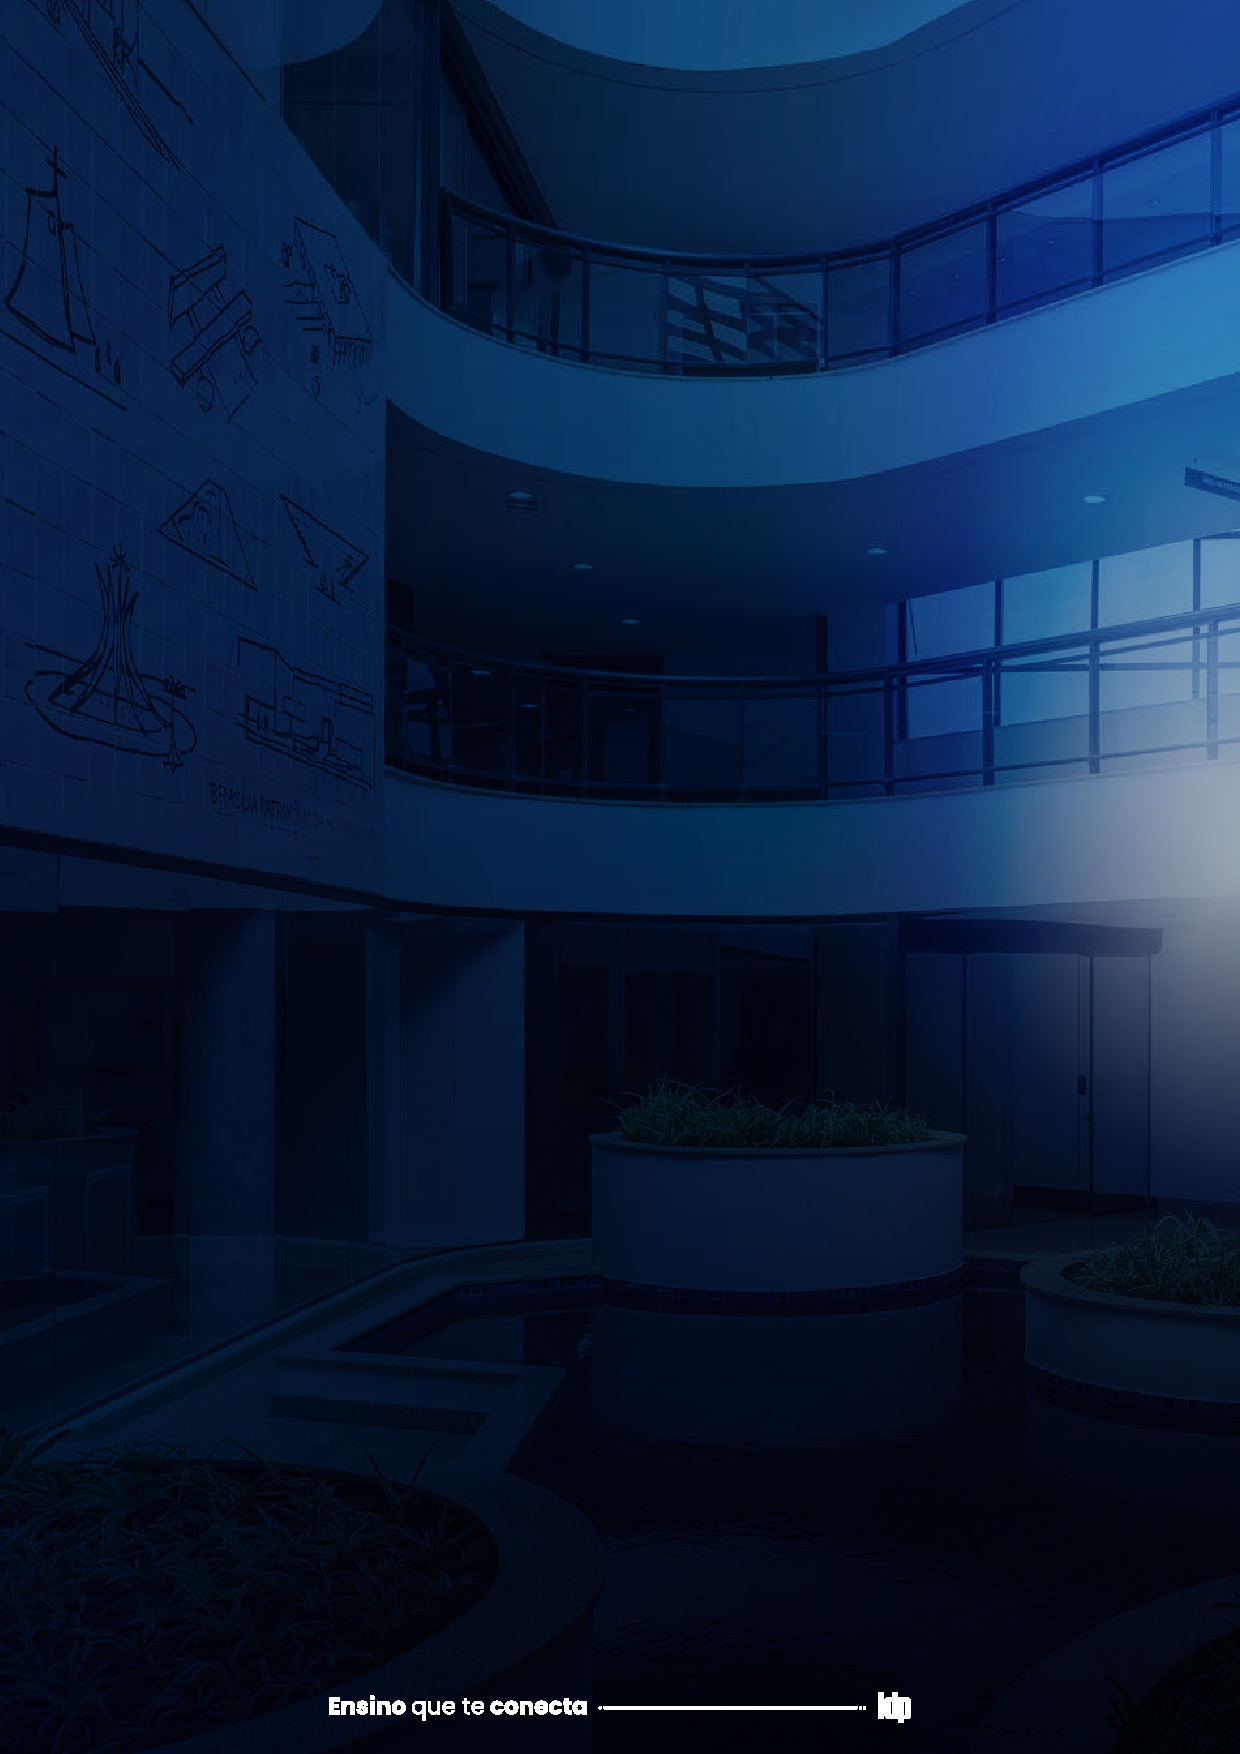
\includegraphics[width=\paperwidth,height=\paperheight]{configs/figuras/capa_secoes.pdf}
        }
    }
     \color{white}

    \vspace*{\fill}
    \begin{center}

    {\fontsize{60}{0}\bfseries\MakeUppercase{Referências}}
    \end{center}
    \vspace*{\fill}

    \refstepcounter{secnum}
    \phantomsection
    \addcontentsline{toc}{section}{Referências}

    \color{black}

    \null
    \clearpage
}

\addto\captionsportuguese{%
  \renewcommand{\refname}{%
    \color{titulos}\bfseries\MakeUppercase{Referências}
  }
}
